\section{Introduzione}
Il progetto è stato realizzato e testato in linguaggio C, per poi essere portato in Cyclone.

Il porting è stato effettuato manualmente ed è consistito principalmente nella
ridefinizione dei tipi puntatore, che rappresentato il cavallo di battaglia di Cyclone
nell’assicurare la type safety.
Si è provato anche il porting semi-automatico, come supporto per la traduzione manuale.

Cyclone è un dialetto safe del C che permette di prevenire diversi tipi di errori e problemi di
sicurezza molto comuni in C come \textbf{buffer overfow, stringhe non terminate e dangling pointers}.
Per ottenere questi risultati si è andato ad aggiunger il garbage collector, che solleva il programmatore dal dover esplicitamente deallocare la memoria con le chiamate free(), riducendo la possibilità di incorrere in dangling pointer o di memoria non deallocata al termine del suo utilizzo.

Altra caratteristica importante di Cyclone sono i qualificatori dei puntatori che meglio
specificano i possibili valori assunti dai puntatori e aggiungono controlli sull'utilizzo degli stessi.

\section{Descrizione del progetto}

L'applicazione scritta in C e successivamente tradotta in Cyclone, consiste in un piccolo programmino in grado di leggere dati da un file, parsarli, fornendo poi una funzionalità di ricerca sui dati contenuti al suo interno.

Nello specifico si è pensato di inserire questa applicazione nell'area break dell'università: infatti, in concomitanza con la macchinettà del caffè gestita in \textit{ASMETA} e il distributore di energy drink prodotto in \textit{Scala}, ho pensato di introdurre un sistema per gestire cartoline, da spedire ai propri cari per gli studenti fuori sede.

Nello specifico è stata realizzata un'interfaccia in grado di funzionare in questo modo:
\begin{itemize}
	\item L'applicazione legge i dati da un file \textit{.txt} in cui sono contenute una serie di cartoline descritte da
	\begin{itemize}
		\item Mittente
		\item Destinatario
		\item Località da cui è stata spedita
	\end{itemize}
	\item Ognuna della informazioni che caratterizza ogni singola cartolina è divisa per mezzo di un carattere delimitatore ("|") che permette alla funzione di \textit{tokenize} di andare ad assegnare le corrette informazioni ad ogni singola cartolina
	\item Una volta letto il file in ingresso, che potrebbe rappresentare l'insieme di tutte le cartoline relativo ad un account su una specifica piattaforma online per la gestione delle cartoline, l'interfaccia permette di eseguire una ricerca:
	\begin{itemize}
		\item \textit{BY SENDER}
		\item \textit{BY RECEIVER}
		\item \textit{BY PLACE}
	\end{itemize}
	stampando poi le cartoline trovate (qualora ce ne fossero).
\end{itemize}

\section{Costrutti Cyclone}
In questa piccola applicazione sono stati due i costrutti principali di Cyclone che sono stati utilizzati:
\begin{itemize}
	\item \textbf{Puntatori}: Cyclone permette l'utilizzo di normali puntatori con le seguenti modifiche rispetto a C
	\begin{itemize}
		\item Controlla se il puntatore è nullo ad ogni de-reference dello stesso (previene \textbf{Segmentation Fault})
		\item Cast vietato da int a puntatore (previene \textbf{Out of Bounds})
		\item Aritmetica dei puntatori vietata (previene \textbf{Buffer Oveflow ~ Overrun e Out of Bounds})
	\end{itemize}
	Ogni puntatore ha inoltre una serie di annotazioni che specificano come deve essere trattato;
	ogni annotazione inizia con un carattere @. 
	
	\item \textbf{Regioni}: vedi sezione ~\ref{sec:regions}
\end{itemize}
\subsection{Puntatori @fat e @thin}
I puntatori sono di default \textbf{@thin}, ovvero non sono in grado di controllare dinamicamente il rispetto dei limiti (bounds) dell’array.

I puntatori \textbf{@fat} (definiti in modo abbreviato con il carattere ?) effettuano invece tale controllo ogni volta che viene utilizzata l’aritmetica dei puntatori.
Essi possono essere pensati come una struttura (struct), per cui i fat pointer permettono l’aritmetica sia in avanti sia all’indietro, con la garanzia di non eccedere i limiti dell’array, come si vede in figura ~\ref{fig:fatStruct}.

\begin{figure}[h]
	\centering
	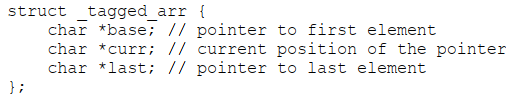
\includegraphics[width=0.5\textwidth]{Immagini/FatPointerStruct.png}
	\caption{@fat pointer visto come una Struct}
	\label{fig:fatStruct}
\end{figure}

Questa tipologia di puntatori, è stata usata diffusamente all'interno del codice Cyclone, sopratutto nella funzione di \textit{tokenize} dove si è ritenuto opportune sfruttare il fatto che i \textit{fat} pointer contengano l'informazione sulla lunghezza, accessibile tramite il comando \textit{numelts}.

\subsection{Puntatori @nullable e @notnull}
\subsubsection{@nullable}
I puntatori sono di default \textbf{@nullable}, ovvero possono assumere valore NULL. Tali puntatori si possono definire anche esplicitamente con *@nullable. 
I puntatori fat possono essere solo @nullable: un puntatore @fat@notnull può essere nullo,

Questa tipologia di identificatori per i puntatori sono stati utilizzati nella fase di apertura del file \textit{.txt}: come si vede in figura ~\ref{fig:nullable}, non  uso di puntatore \textit{@notnull} per garantire le gestione del caso in cui non si riesca ad aprire il file di testo, tramite un print di errore.

\begin{figure}[h]
	\centering
	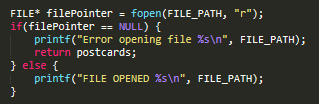
\includegraphics[width=0.5\textwidth]{Immagini/NullablePointerFile.png}
	\caption{Gestione pointer nullable}
	\label{fig:nullable}
\end{figure}

\subsubsection{@notnull}
I puntatori @notnull non possono invece essere nulli, ovvero non è possibile assegnare loro il
valore NULL. Essi possono essere definiti in modo abbreviato con il carattere @.
I puntatori non nulli sono sicuramente i più utilizzati, sia perché non introducono l’overhead
del controllo di non-nullità (che viene garantita a compile-time), sia perché nella quasi totalità
dei casi un puntatore è utilizzato per operare sull’oggetto puntato e non per verificare se tale
oggetto esiste, quindi si dà per scontato che esso esista.

Questa tipologia di puntatore è stata largamente utilizzata nper quanto riguarda le stringhe, relative alla struttura \textit{postcard}.

\subsection{Regioni}
\label{sec:regions}
Per evitare dangling pointers, Cyclone impone che ogni puntatore dichiari in quale area della
memoria punti. L’area (region) in cui punta può essere un particolare record di attivazione
sullo stack, lo heap o una regione di stack allocata dinamicamente. Ogni puntatore può puntare
solo a regioni che hanno una vita uguale o più lunga di quella della regione dichiarata; ad
esempio, un puntatore allo heap può puntare solo allo heap, un puntatore al record di
attivazione di una funzione può puntare a quel record, ai record dei chiamanti della funzione o
allo heap, ma non può puntare a record di funzioni chiamate

Per indicare esplicitamente una regione, si deve annotare il puntatore con @region(`r) o
@effect(`r) o semplicemente `r, dove r è il nome di un’opportuna regione o un semplice
segnaposto. `H rappresenta lo heap.